\section{Define Logical Architecture}
\label{section:define-logical-architecture}

Nine implementation-independent capabilities realize F01--F08 \citep[Sec.~17.3.4]{friedenthal2014practical}. Learning, finances, RAM, credibility, software and technician concerns extend the response beyond evidence custody. El Hachimi et al. inform mission-driven sizing, component and thermal/EMC decisions, protection and telemetry checks \citep[Secs.~2--5 and~8.1.6--8.1.7]{handpicked-0003}. The Handbook informs coordinated requirements, budgets, interfaces and verification planning \citep[Secs.~I.3--I.4]{aguado2021cubesatse}. Their EPS results remain case-specific.

\begin{figure}[!htbp]
\centering
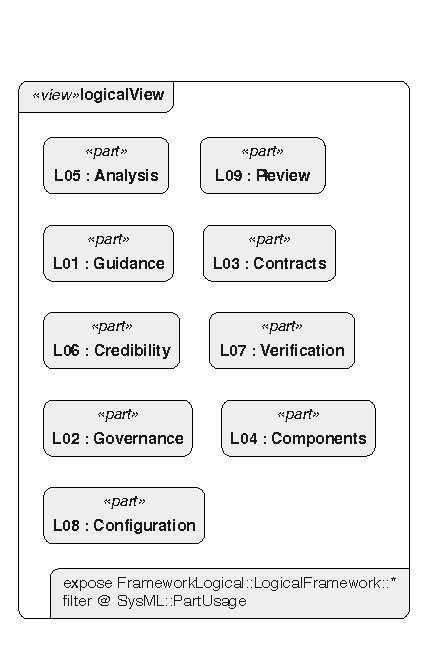
\includegraphics[width=\linewidth,height=0.74\textheight,keepaspectratio]{figures/sysml/logical/sysml-defined-view-reportviews-logicalview.pdf}
\caption{Nine logical capabilities of the framework.}
\label{fig:framework-logical}
\end{figure}

\subsection{Responsibilities and allocations}

Each FR has one primary owner below. Supporting owners and typed record fields remain in the registry. These capabilities imply no executable or node count. Allocations state design responsibility.
{\small
\setlength{\tabcolsep}{4pt}
\setlength{\parskip}{0pt}
\setlength{\LTpre}{0.4\baselineskip}
\setlength{\LTpost}{0.4\baselineskip}
\renewcommand{\arraystretch}{1.06}
\begin{longtable}{@{}>{\raggedright\arraybackslash}p{\dimexpr0.31\linewidth-1.24\tabcolsep\relax}>{\raggedright\arraybackslash}p{\dimexpr0.51\linewidth-2.04\tabcolsep\relax}>{\raggedright\arraybackslash}p{\dimexpr0.18\linewidth-0.72\tabcolsep\relax}@{}}
\caption{Logical records, required/provided services and primary leaf allocation. FR numbers appear in the last column.}\label{tab:framework-logical}\\
\toprule
\textbf{Capability} & \textbf{Records and exchanges} & \textbf{Primary FR} \\
\midrule
\endfirsthead
\caption[]{Logical records, required/provided services and primary leaf allocation. FR numbers appear in the last column. (continued).}\\
\toprule
\textbf{Capability} & \textbf{Records and exchanges} & \textbf{Primary FR} \\
\midrule
\endhead
\bottomrule
\endfoot
L01\par Engineering guidance and knowledge & Sourced methods, templates, examples and lessons. Case goals/findings enter. Applicable guidance returns. & 02, 03 \\
L02\par Needs, requirements and decision governance & Requirements, decisions, links, impacts and dispositions. Domain revisions enter. Derived obligations and affected-claim/change records return. & 01, 04, 05, 06, 11, 17, 26 \\
L03\par Architecture and service contracts & Generic/case structure, interfaces, modes and software contracts. Requirements/properties enter. Mappings, dictionaries and sequence specifications return. & 15, 18, 33, 34, 35, 36 \\
L04\par Component and lifecycle characterization & Component facts, occurrence quantities, BOMs, quotes and failures. Architecture/source updates enter. Estimates and RAM representations return with unknowns. & 12, 13, 27 \\
L05\par Scenario and analysis orchestration & Analysis plans, run packages and replay instructions. Frozen inputs/models/criteria enter. Dynamic, virtual, battery/policy and common-basis results return. & 10, 14, 16, 19, 20, 23, 24 \\
L06\par Model credibility and observation reconciliation & Validity, calibration/validation, observation quality and timing. Models/results/data enter. Residuals, alternatives and update proposals return. & 21, 22, 25, 31, 32 \\
L07\par Verification specification and safety & Verification specifications, proposals and scoped verdicts. Criteria, DUT/equipment and admissible results enter. Procedures, readiness and residual obligations return. & 28, 29, 30 \\
L08\par Information and configuration authority & Identities, schemas, registrations, manifests and custody. Identified artifacts enter. Checked transfers, baselines and reconstruction packages return. & 07, 08, 09 \\
L09\par Case workspace and technical review & Case declarations, findings, environment/evaluation records. Evidence/guidance enter. Views, reviews, adoption and two-case outcomes return. & 37, 38, 39, 40 \\
\end{longtable}
}

\subsection{Typed exchanges, authority and feedback}
{\small
\setlength{\tabcolsep}{4pt}
\setlength{\parskip}{0pt}
\setlength{\LTpre}{0.4\baselineskip}
\setlength{\LTpost}{0.4\baselineskip}
\renewcommand{\arraystretch}{1.06}
\begin{longtable}{@{}>{\raggedright\arraybackslash}p{\dimexpr0.32\linewidth-0.64\tabcolsep\relax}>{\raggedright\arraybackslash}p{\dimexpr0.68\linewidth-1.36\tabcolsep\relax}@{}}
\caption{Grouped internal contracts.}\label{tab:framework-logical-exchanges}\\
\toprule
\textbf{Participants} & \textbf{Receiving obligation} \\
\midrule
\endfirsthead
\caption[]{Grouped internal contracts. (continued).}\\
\toprule
\textbf{Participants} & \textbf{Receiving obligation} \\
\midrule
\endhead
\bottomrule
\endfoot
All $\leftrightarrow$ L08 & Registration, transfer verdict, exact manifest and reconstruction. Check envelope/semantics/provenance and preserve rejected/prior revisions. \\
L02 $\leftrightarrow$ L03/L04/L06/L07 & Requirements, criteria, impact and domain revision proposals. Resolve dependencies and retain stale/unresolved evidence. \\
L03/L04/L06/L07 $\rightarrow$ L05 & Occurrences, characterization, failure dependencies, applicable models and verification criteria freeze the run. Software mappings also drive sequence/resource checks. \\
L05 $\rightarrow$ L06 $\rightarrow$ L07 $\rightarrow$ L02 & Raw run, credibility assessment, admissible verdict and affected-claim status. Supplied observations return through proposed parameter/design updates. \\
L01/L09 $\leftrightarrow$ domain owners & Guidance, baseline-linked reviews, findings and lessons. Apply tailoring, return findings to owners and separate local learning from general source claims. \\
\end{longtable}
}

L08 owns accepted manifests and common identity/schema rules. Domain owners retain semantic authority over requirements (L02), architecture/services (L03), characterization (L04), credibility/observations (L06), verification (L07), knowledge (L01) and case/review declarations (L09). References avoid competing field copies. Generated dictionaries, scaffolds, solver inputs and views identify source/transformation revisions. Mission behavior and deployment remain separate software artifacts \citep[Secs.~3--5]{review-0853}.

Quantity, sign, reference-frame, clock and validity contracts address model, degradation, sensor and timing effects \citep[Secs.~4.1--4.2 and~6]{review-1251}. Numerical step size proves no real-time suitability \citep[Sec.~3]{review-0573}. SC01 follows guidance and definition, analysis, credibility assessment, verification and review. SC02 threads impact through domain revisions and reanalysis. SC03 threads failed observations through updates and safe proposals. Design change, observation reconciliation and reviewed learning share L08 revision control. They never silently overwrite earlier evidence or actuate hardware.
